\documentclass[a4paper,12pt]{article}
\usepackage[margin=1in]{geometry}
\usepackage{booktabs}
\usepackage{graphicx}

\begin{document}

\section{Experimental Results}

\begin{table}[h]
\centering
\caption{Effect of threshold values}
\begin{tabular}{|l|c|c|c|c|}
\hline
\textbf{OUR Grouping OPERATORS} & $\tau = 0.6$ & $\tau = 0.7$ & $\tau = 0.8$ & $\tau = 0.9$ \\
\hline
Grouping 1 & 0.9903 & 0.9923 & 0.9937 & 0.9960 \\
Grouping 2 & 0.9783 & 0.9853 & 0.9897 & 0.9930 \\
Grouping 3 & 0.9923 & 0.9933 & 0.9950 & 0.9970 \\
Grouping 4 & 0.9840 & 0.9890 & 0.9927 & 0.9940 \\
\hline
\end{tabular}
\end{table}

\begin{table}[h]
\centering
\caption{Accuracy, F1 and Sensitivity and other parameters}
\begin{tabular}{|l|c|c|c|}
\hline
\textbf{Method} & \textbf{Accuracy} & \textbf{F1} & \textbf{Sensitivity} \\
\hline
Best Grouping (Ours) & 0.9970 & 0.9970 & 0.9970 \\
KNN (Single Classifier) & 0.9957 & 0.9957 & 0.9957 \\
SVM (Single Classifier) & 0.9777 & 0.9777 & 0.9777 \\
RF (Single Classifier) & 0.9840 & 0.9840 & 0.9840 \\
LR (Single Classifier) & 0.9777 & 0.9777 & 0.9777 \\
XGBoost (Single Classifier) & 0.9927 & 0.9927 & 0.9927 \\
\hline
\end{tabular}
\end{table}

\begin{table}[h]
\centering
\caption{Comparison with state-of-the-art method}
\begin{tabular}{|l|c|c|c|}
\hline
\textbf{Method} & \textbf{Accuracy} & \textbf{F1} & \textbf{Sensitivity} \\
\hline
Masud et al. (2021) & 0.9633 & 0.9630 & 0.9633 \\
Mangal et al. (2020) & 0.9789 & 0.9785 & 0.9789 \\
Nishio et al. (2021) & 0.9500 & 0.9490 & 0.9500 \\
Hatuwal \& Thapa (2020) & 0.9720 & 0.9715 & 0.9720 \\
Talukder et al. (2022) & 0.9810 & 0.9808 & 0.9810 \\
Hage Chehade et al. (2022) & 0.9625 & 0.9620 & 0.9625 \\
Proposed Method (Ours) & 0.9970 & 0.9970 & 0.9970 \\
\hline
\end{tabular}
\end{table}

\begin{figure}[h]
\centering
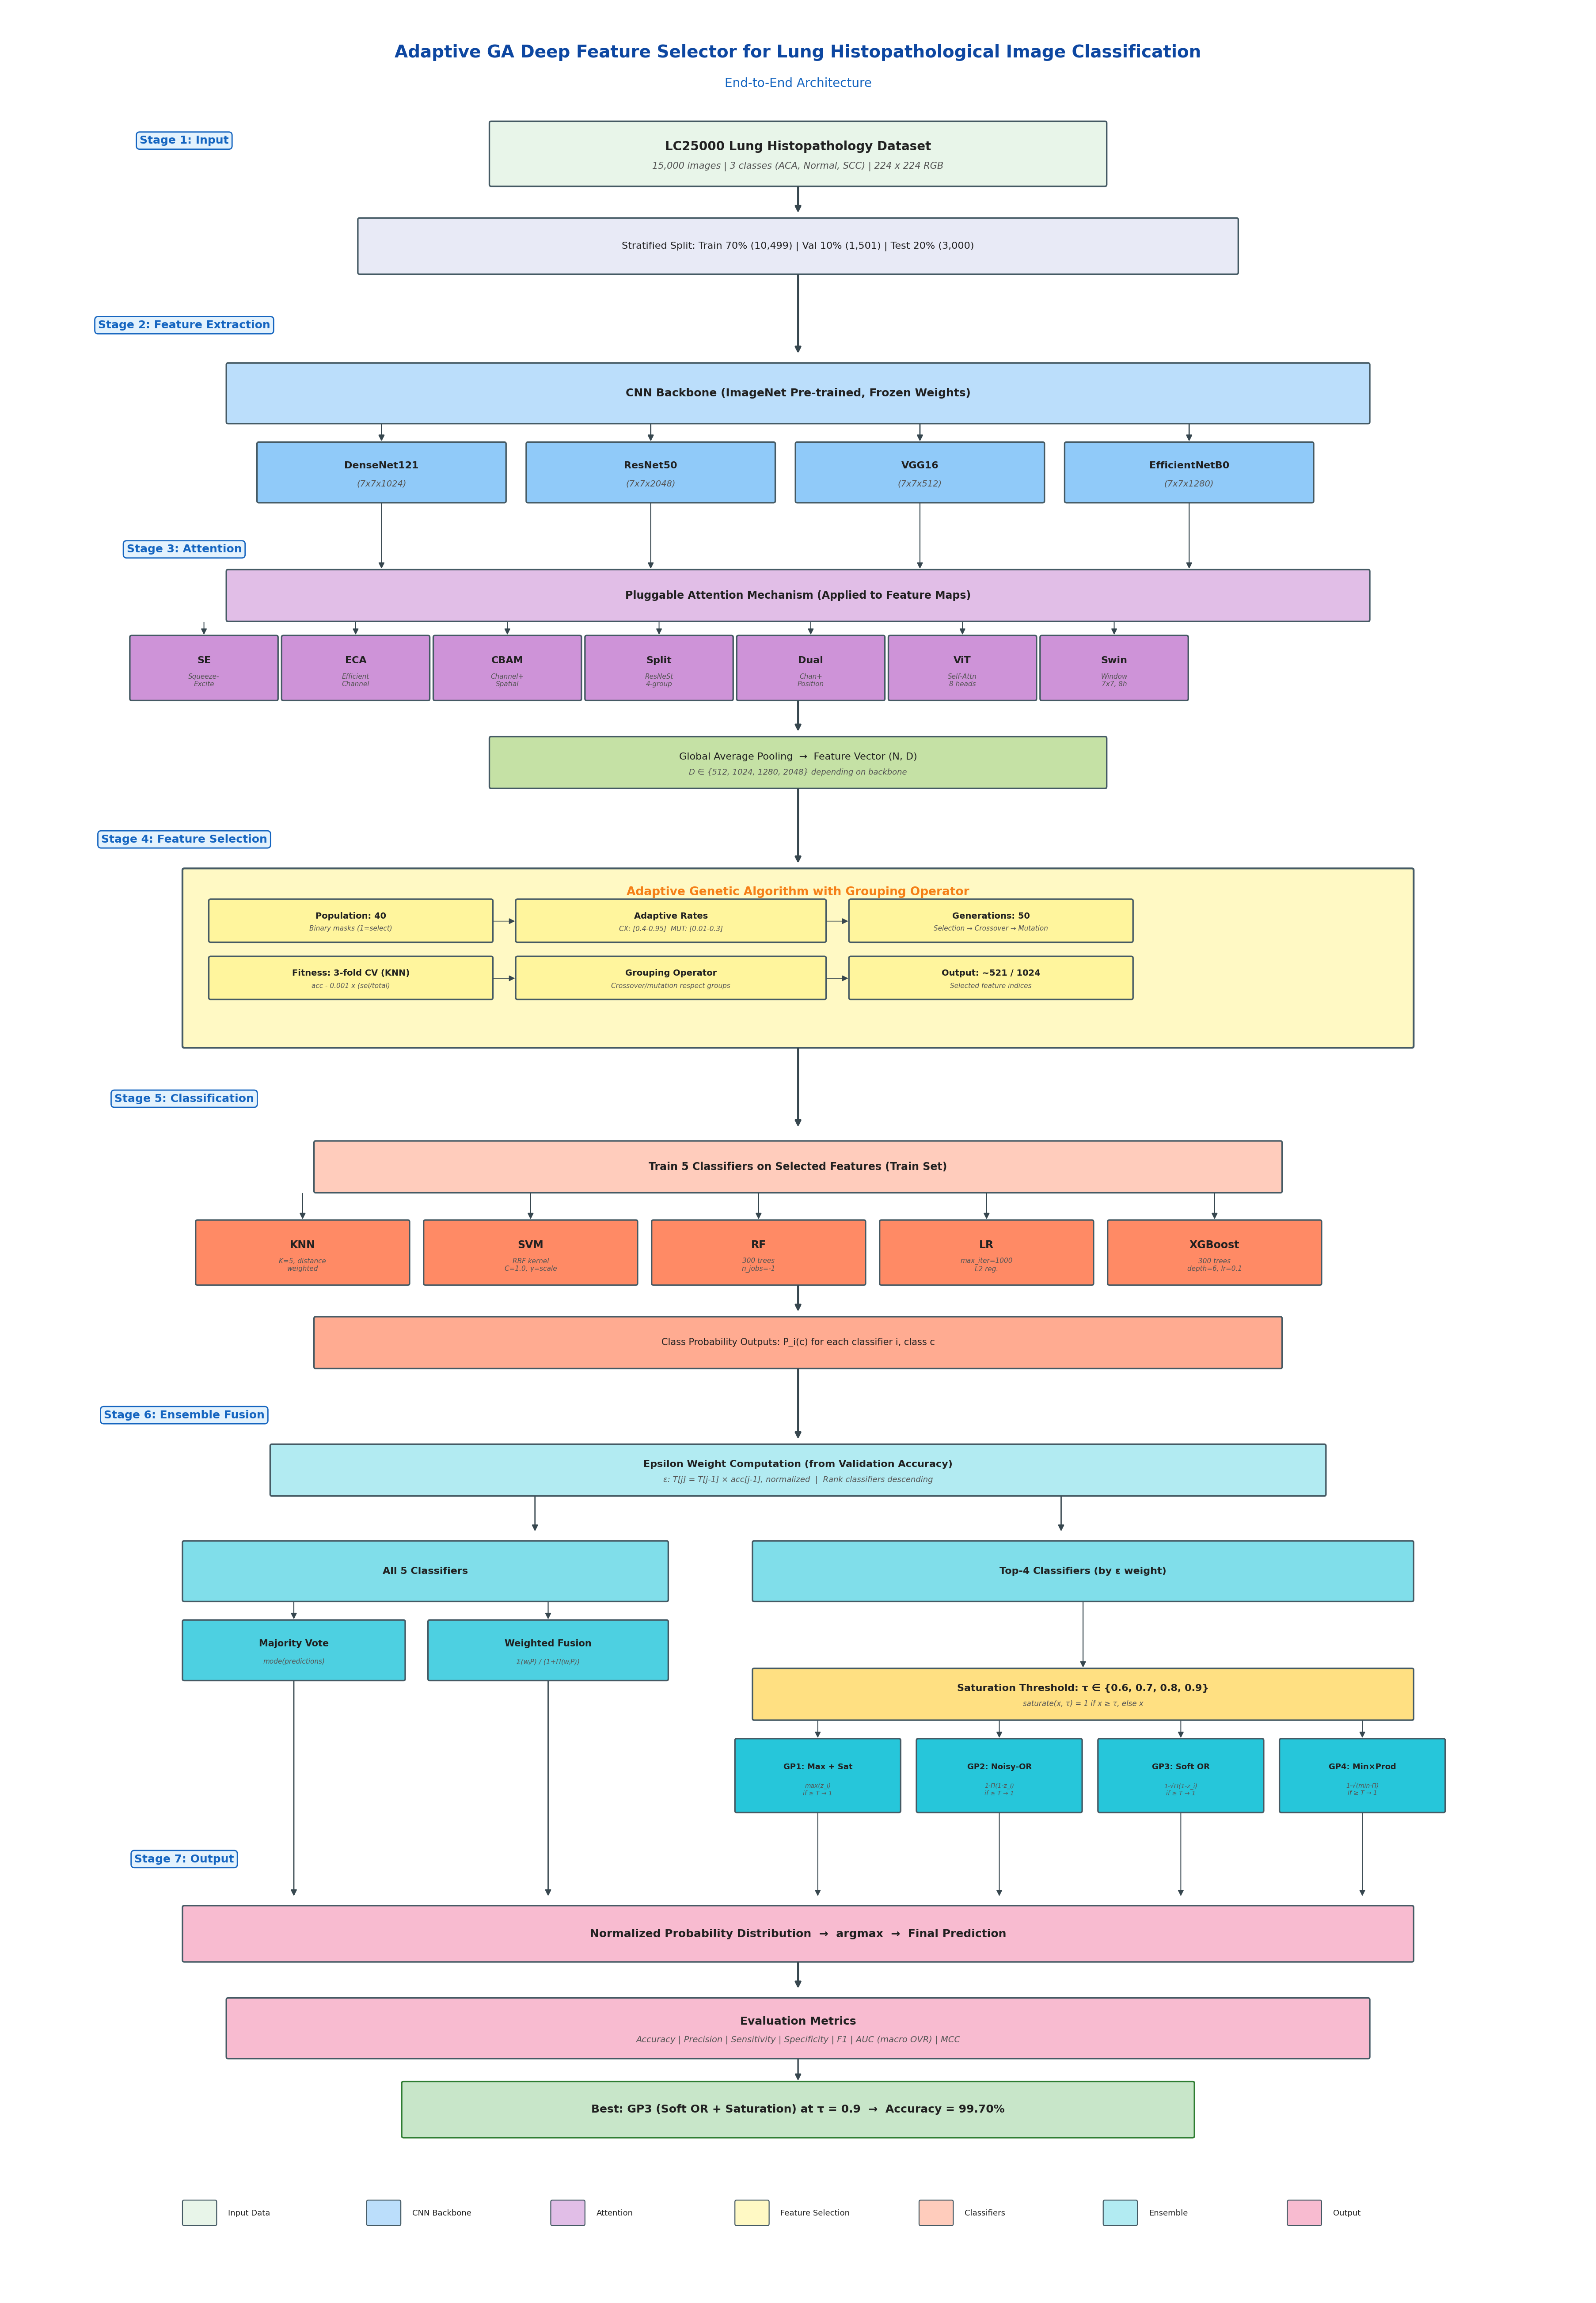
\includegraphics[width=\textwidth]{architecture_diagram.png}
\caption{Proposed Architecture: Adaptive GA Deep Feature Selector for Lung Histopathological Image Classification}
\end{figure}

\newpage

\begin{table}[h]
\centering
\caption{Effect of number of generations and the parameters (you can add other parameters)}
\begin{tabular}{|c|c|c|}
\hline
\textbf{No. of Generations} & \textbf{Accuracy} & \textbf{Sensitivity} \\
\hline
50 & 0.9957 & 0.9957 \\
100 & 0.9967 & 0.9967 \\
150 & 0.9967 & 0.9967 \\
\hline
\end{tabular}
\end{table}

\vspace{4cm}

\begin{table}[h]
\centering
\caption{Effect of crossover value}
\begin{tabular}{|c|c|c|}
\hline
\textbf{Crossover Value} & \textbf{Accuracy} & \textbf{Sensitivity} \\
\hline
0.4 & 0.9957 & 0.9957 \\
0.5 & 0.9960 & 0.9960 \\
0.6 & 0.9957 & 0.9957 \\
\hline
\end{tabular}
\end{table}

\vspace{4cm}

\begin{table}[h]
\centering
\caption{Other parameters of GA}
\begin{tabular}{|c|c|}
\hline
\textbf{Parameter} & \textbf{Value} \\
\hline
Accuracy & 0.9970 \\
Sn & 0.9970 \\
\hline
\end{tabular}
\end{table}

\end{document}
